\documentclass[12pt]{article}

\usepackage{geometry}                % See geometry.pdf to learn the layout options. There are lots.
\usepackage{fullpage}
\usepackage{graphicx}
\usepackage{amsmath}
\usepackage{amssymb}
\usepackage{epstopdf}

\newcommand{\real}{{\mathbb{R}}}
\newcommand{\Id}{{\mathbb{I}}}
\newcommand{\xdot}{\dot{x}}
\newcommand{\pard}[2]{\frac{\partial #1}{\partial #2}}

\title{Numerical Implementation of the Doyle-Fuller-Newman (DFN) Model}
\author{{\normalsize Prof. Scott Moura} $\mid$ {\normalsize Energy, Controls, and Applications Lab (eCAL) $\mid$ UC Berkeley}}
\date{{\normalsize IN PROGRESS $\mid$ \today}}                                           % Activate to display a given date or no date

%%%%%%%%%%%%%%%%%%%%%%%%%%%
\begin{document}
\maketitle

%\section{}
%\subsection{}

In this note we document the numerical implementation of the DFN model.

%%%%%%%%%%%%%%%%%%%%%%%%%%%
\section{Doyle-Fuller-Newman Model}\label{sec:dfn}

We consider the Doyle-Fuller-Newman (DFN) model in Fig. \ref{fig:dfn-schematic} to predict the evolution of lithium concentration in the solid $c_{s}^{\pm}(x,r,t)$, lithium concentration in the electrolyte $c_{e}(x,t)$, solid electric potential $\phi_{s}^{\pm}(x,t)$, electrolyte electric potential $\phi_{e}(x,t)$, ionic current $i_{e}^{\pm}(x,t)$, molar ion fluxes $j_{n}^{\pm}(x,t)$, and bulk cell temperature $T(t)$ \cite{Thomas2002}. The governing equations are given by
\begin{eqnarray}
	\frac{\partial c_{s}^{\pm}}{\partial t}(x,r,t) &=& \frac{1}{r^{2}} \frac{\partial}{\partial r} \left[ D_{s}^{\pm} r^{2} \frac{\partial c_{s}^{\pm}}{\partial r}(x,r,t) \right], \label{eqn:cs} \\
	\frac{\partial c_{e}}{\partial t}(x,t) &=& \frac{\partial}{\partial x} \left[ D_{e} \frac{\partial c_{e}}{\partial x}(x,t) + \frac{1 - t_{c}^{0}}{\varepsilon_{e} F} i_{e}^{\pm}(x,t) \right], \label{eqn:ce} \\
	0 &=& \frac{\partial \phi_{s}^{\pm}}{\partial x}(x,t) - \frac{i_{e}^{\pm}(x,t) - I(t)}{\sigma^{\pm}}, \label{eqn:phis} \\
	0 &=& \frac{\partial \phi_{e}}{\partial x}(x,t) + \frac{i_{e}^{\pm}(x,t)}{\kappa} - \frac{2RT}{F}(1 - t_{c}^{0}) \times \left(1 + \frac{d \ln f_{c/a}}{d \ln c_{e}}(x,t) \right) \frac{\partial \ln c_{e}}{\partial x}(x,t), \label{eqn:phie} \quad \\
	0 &=& \frac{\partial i_{e}^{\pm}}{\partial x}(x,t) - a_{s} F j_{n}^{\pm}(x,t), \label{eqn:ie} \\
	0 &=& \frac{1}{F} i_{0}^{\pm}(x,t) \left[e^{\frac{\alpha_{a}F}{RT} \eta^{\pm}(x,t)} - e^{-\frac{\alpha_{c}F}{RT} \eta^{\pm}(x,t)} \right] - j_{n}^{\pm}(x,t), \label{eqn:bv} \\
	\rho^{\textrm{avg}} c_{P} \frac{dT}{dt}(t) &=& h_{\textrm{cell}} \left[ T_{\textrm{amb}}(t) - T(t) \right] + I(t) V(t) -\int_{0^{-}}^{0^{+}} a_{s} F j_{n}(x,t) \Delta T(x,t) dx,
\end{eqnarray}
where $D_{e}, \kappa, f_{c/a}$ are functions of $c_{e}(x,t)$ and
\begin{eqnarray}
	i_{0}^{\pm}(x,t) &=& k^{\pm}  \left[ c_{ss}^{\pm}(x,t) \right]^{\alpha_{c}} \left[c_{e}(x,t) \left(c_{s,\max}^{\pm} - c_{ss}^{\pm}(x,t)  \right) \right]^{\alpha_{a}}, \label{eqn:i0} \\
	\eta^{\pm}(x,t) &=& \phi_{s}^{\pm}(x,t) - \phi_{e}(x,t) - U^{\pm}(c_{ss}^{\pm}(x,t)) - F R_{f}^{\pm} j_{n}^{\pm}(x,t), \label{eqn:eta} \\
	c_{ss}^{\pm}(x,t) &=& c_{s}^{\pm}(x,R_{s}^{\pm},t), \label{eqn:css} \\
	\Delta T(x,t) &=& U^{\pm}(\overline{c}^{\pm}_{s}(x,t)) - T(t) \frac{\partial U^{\pm}}{\partial T}(\overline{c}^{\pm}_{s}(x,t)), \\
	\overline{c}_{s}^{\pm}(x,t) &=& \frac{3}{(R_{s}^{\pm})^{3}} \int_{0}^{R_{s}^{\pm}} r^{2} c_{s}^{\pm}(x,r,t) dr \label{eqn:cbulk}
\end{eqnarray}

\begin{figure}[t]
  \centering
  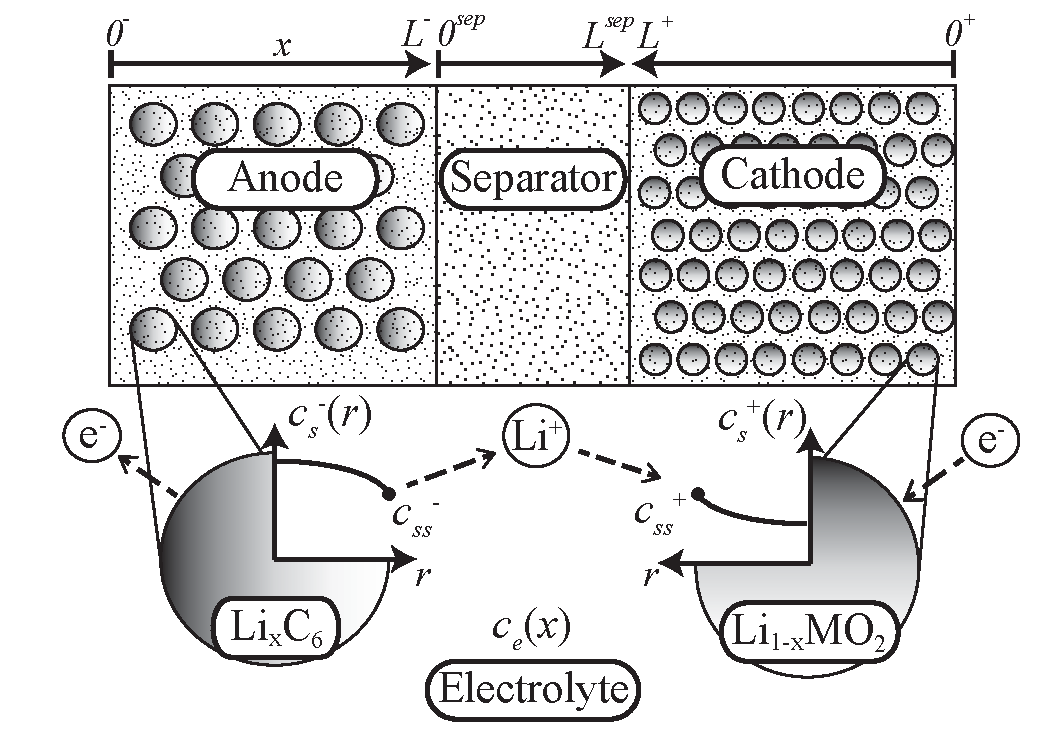
\includegraphics[trim = 0.4in 0.1in 0.15in 0.05in, clip, width=4.5in]{dfn-schematic.pdf}
  \caption{Schematic of the Doyle-Fuller-Newman model \cite{Thomas2002}. The model considers two phases: the solid and electrolyte. In the solid, states evolve in the $x$ and $r$ dimensions. In the electrolyte, states evolve in the $x$ dimension only. The cell is divided into three regions: anode, separator, and cathode.}
  \label{fig:dfn-schematic}
\end{figure}

Along with these equations are corresponding boundary and initial conditions. The boundary conditions for the solid-phase diffusion PDE (\ref{eqn:cs}) are
\begin{eqnarray}
	\frac{\partial c_{s}^{\pm}}{\partial r}(x,0,t) &=& 0, \\
	\frac{\partial c_{s}^{\pm}}{\partial r}(x,R_{s}^{\pm},t) &=& -\frac{1}{D_{s}^{\pm}} j_{n}^{\pm}.
\end{eqnarray}
The boundary conditions for the electrolyte-phase diffusion PDE (\ref{eqn:ce}) are given by
\begin{align}
	\pard{c_{e}}{x}(0^{-},t) &= \pard{c_{e}}{x}(0^{+},t) = 0, \label{eqn:ce-bc1} \\
	\varepsilon_{e}^{-} D_{e}^{-}(L^{-}) \pard{c_{e}}{x}(L^{-},t) &= \varepsilon_{e}^{\textrm{sep}}D_{e}^{\textrm{sep}}(0^{\textrm{sep}}) \pard{c_{e}}{x}(0^{\textrm{sep}},t), \\
	\varepsilon_{e}^{\textrm{sep}}D_{e}^{\textrm{sep}}(L^{\textrm{sep}}) \pard{c_{e}}{x}(L^{\textrm{sep}},t) &= \varepsilon_{e}^{+} D_{e}^{+}(L^{+}) \pard{c_{e}}{x}(L^{+},t), \\
	c_{e}(L^{-},t) &= c_{e}(0^{\textrm{sep}},t), \\
	c_{e}(L^{\textrm{sep}},t) &= c_{e}(0^+,t). \label{eqn:ce-bc5}
\end{align}
The boundary conditions for the solid-phase potential ODE (\ref{eqn:phis}) are given by
\begin{equation}\label{eqn:phis-bc}
	\pard{\phi_{s}^{-}}{x}(L^{-},t) = \pard{\phi_{s}^{+}}{x}(L^{+},t) = 0.
\end{equation}
The boundary conditions for the electrolyte-phase potential ODE (\ref{eqn:phie}) are given by
\begin{eqnarray}
	\phi_{e}(0^{-},t) &=& 0, \\
	\phi_{e}(L^{-},t) &=& \phi_{e}(0^{\textrm{sep}},t), \\
	\phi_{e}(L^{\textrm{sep}},t) &=& \phi_{e}(L^+,t).
\end{eqnarray}
The boundary conditions for the ionic current ODE (\ref{eqn:ie}) are given by
\begin{equation}\label{eqn:ie-bcs}
	i_{e}^{-}(0^{-},t) = i_{e}^{+}(0^+,t) = 0
\end{equation}
and also note that $i_{e}(x,t) = I(t)$ for $x \in [0^{\textrm{sep}}, L^{\textrm{sep}}]$.

The input to the model is the applied current density $I(t)$, and the output is the voltage measured across the current collectors
\begin{equation}\label{eqn:voltage}
	V(t) = \phi^{+}_{s}(0^{+},t) - \phi_{s}^{-}(0^{-},t)
\end{equation}
Further details, including notation definitions, can be found in \cite{Thomas2002,Chaturvedi2010}.

%%%%%%%%%%%%%%%%%%%%%%%%%%%
\section{Time-stepping}\label{sec:time-step}

Ultimately, the equations are discretized to produce a DAE in the following format:
\begin{eqnarray}
	\xdot &=& f(x, z, u), \label{eqn:dae1} \\
	0 &=& g(x,z,u) \label{eqn:dae2}
\end{eqnarray}
with initial conditions $x(0), z(0)$ that are consistent. That is, they verify (\ref{eqn:dae2}). The time-stepping is done by solving the nonlinear equation
\begin{align}
	 0 &= F(x(t + \Delta t), z(t + \Delta t)), \label{eqn:cfn1} \\
0 &= \left[
\begin{array}{c}
  x(t) - x(t+\Delta t) + \frac{1}{2} \Delta t \left[ f(x(t), z(t), u(t)) + f(x(t+\Delta t), z(t+\Delta t), u(t+\Delta t)) \right] \\
  g\left(x(t+\Delta t), z(t+\Delta t), u(t + \Delta t) \right)
\end{array}
\right] \label{eqn:cfn2}
\end{align} 
for $x(t+\Delta t), z(t+\Delta t)$. The function \texttt{cfn\_dfn.m} returns the solution $\left(x(t+\Delta t), z(t+\Delta t)\right)$ of (\ref{eqn:cfn1})-(\ref{eqn:cfn2}), given $x(t), z(t), u(t), u(t+\Delta t)$. Note that we solve (\ref{eqn:cfn1})-(\ref{eqn:cfn2}) using Newton's method, meaning analytic Jacobians of $F(\cdot, \cdot)$ are required w.r.t. $x,z$.
\begin{align}
J &=
\left[
\begin{array}{cc}
 F^{1}_{x} & F^{1}_{z}  \\
 F^{2}_{x} & F^{2}_{z}
\end{array}
\right] \\
&= 
\left[
\begin{array}{cc}
 -I + \frac{1}{2} \Delta t \cdot \frac{\partial f}{\partial x}(x(t+\Delta t),z(t+\Delta t),u(t+\Delta t)) & \frac{1}{2} \Delta t \cdot \frac{\partial f}{\partial z}(x(t+\Delta t),z(t+\Delta t),u(t+\Delta t))  \\
 \frac{\partial g}{\partial x}(x(t+\Delta t),z(t+\Delta t),u(t+\Delta t)) & \frac{\partial g}{\partial z}(x(t+\Delta t),z(t+\Delta t),u(t+\Delta t))
\end{array}
\right]
\end{align}

%%%%%%%%%%%%%%%%%%%%%%%%%%%
\section{DAEs}\label{sec:daes}
To perform the time-stepping in the previous section, we must compute functions $f(x,z,u)$ and $g(x,z,u)$. These functions, which represent the RHS of (\ref{eqn:dae1})-(\ref{eqn:dae2}), are calculated by the Matlab function \texttt{dae\_dfn.m}, given the inputs $x,z,u$. The role of variables $x,z,u$ are played by the DFN variables shown in Table \ref{tbl:dae-notation}.

\begin{table}[h]
\caption{DAE notation for DFN states in Matlab Code}
\begin{center}
\begin{tabular}{c|c}
\hline \hline
\textbf{DAE Variable} & \textbf{DFN Variable} \\
\hline
$x$ & $c_{s}^{-}, c_{s}^{+}, c_{e} = [c_{e}^{-}, c_{e}^{sep}, c_{e}^{+}], T$ \\
$z$ & $\phi_{s}^{-}, \phi_{s}^{+}, i_{e}^{-}, i_{e}^{+}, \phi_{e} = [\phi_{e}^{-}, \phi_{e}^{sep}, \phi_{e}^{+}], j_{n}^{-}, j_{p}^{+}$ \\
$u$ & $I$ \\
\hline \hline
\end{tabular}
\end{center}
\label{tbl:dae-notation}
\end{table}%

In the subsequent sections, we go through each DFN variable listed in Table \ref{tbl:dae-notation} and document its numerical implementation.

%%%%%%%%%%%%%%%%%%%%%%%%%%%
\section{Solid Concentration, $c_{s}^{-}, c_{s}^{+}$}\label{sec:cs}
[DONE] The PDEs (\ref{eqn:cs}) governing Fickian diffusion in the solid phase are implemented using third order Pad\'{e} approximations of the two transfer functions from $j_{n}^{\pm}$ to $c_{ss}^{\pm}$ and $\overline{c}_{s}^{\pm}$. 
\begin{eqnarray}
	\frac{C_{ss}^{\pm}(s)}{J_{n}^{\pm}(s)} &=& \frac{-\frac{21}{R_{s}^{\pm}}s^{2} -\frac{1260 D_{s}^{\pm}}{(R_{s}^{\pm})^{3}}s -\frac{10395 (D_{s}^{\pm})^{2}}{ (R_{s}^{\pm})^{4} }  }{s^{3} + \frac{189 D_{s}^{\pm}}{(R_{s}^{\pm})^{2}} s^{2} + \frac{3465 (D_{s}^{\pm})^{2}}{(R_{s}^{\pm})^{4}} s }, \\
	\frac{\overline{C}_{s}^{\pm}(s)}{J_{n}^{\pm}(s)} &=& \frac{-3 R_{s}^{\pm}}{s}.
\end{eqnarray}
These transfer functions are converted into controllable canonical state-space form , thus producing the subsystem:
\begin{eqnarray}
\frac{d}{dt}
\left[
\begin{array}{c}
 c_{s1}^{\pm}(t) \\
 c_{s2}^{\pm}(t) \\
 c_{s3}^{\pm}(t)
\end{array}
\right]
&=&
\left[
\begin{array}{ccc}
 0 & 1  & 0  \\
 0 & 0  & 1  \\
 0 & -\frac{3465 (D_{s}^{\pm})^{2}}{(R_{s}^{\pm})^{4}}  & -\frac{189 D_{s}^{\pm}}{(R_{s}^{\pm})^{2}}  
\end{array}
\right]
\left[
\begin{array}{c}
 c_{s1}^{\pm}(t) \\
 c_{s2}^{\pm}(t) \\
 c_{s3}^{\pm}(t)
\end{array}
\right] + 
\left[
\begin{array}{c}
 0 \\
 0 \\
 1
\end{array}
\right] j_{n}^{\pm}(t) \\
\left[
\begin{array}{c}
 c_{ss}^{\pm}(t) \\
 \overline{c}_{s}^{\pm}(t)
\end{array}
\right] &=& 
\left[
\begin{array}{ccc}
 -\frac{10395 (D_{s}^{\pm})^{2}}{(R_{s}^{\pm})^{5}} & -\frac{1260 D_{s}^{\pm}}{(R_{s}^{\pm})^{3}}  & -\frac{21}{R_{s}^{\pm}}  \\
 -\frac{3}{R_{s}^{\pm}} \cdot \frac{3465 (D_{s}^{\pm})^{2}}{(R_{s}^{\pm})^{4}} & -\frac{3}{R_{s}^{\pm}} \cdot \frac{189 D_{s}^{\pm}}{(R_{s}^{\pm})^{2}} & -\frac{3}{R_{s}^{\pm}} \cdot 1
\end{array}
\right]
\left[
\begin{array}{c}
 c_{s1}^{\pm}(t) \\
 c_{s2}^{\pm}(t) \\
 c_{s3}^{\pm}(t)
\end{array}
\right]
\end{eqnarray}
for each discrete point in $x$.

%%%%%%%%%%%%%%%%%%%%%%%%%%%
\section{Electrolyte Concentration, $c_{e}$}\label{sec:ce}
[DONE] The electrolyte concentration is implemented using the central difference method, which ultimately produces the matrix differential equation:
\begin{equation}
	\frac{d}{dt} c_{e}(t) = A_{ce}(c_{e,x}) \cdot c_{e}(t) + B_{ce}(c_{e,x}) \cdot i_{e,x}(t)
\end{equation}
where $c_{e}, i_{e,x}$ are vectors whose elements represent discrete points along the $x$-dimension of the DFN model. In particular $i_{e,x}$ and $c_{e,x}$ represent the entire electrolyte current and concentration, respectively, across the entire battery, including boundary values,
\begin{eqnarray}
	i_{e,x}(t) &=& \left[0, \ i_{e}^{-}(x,t), \ I(x,t), \ i_{e}^{+}(x,t), \ 0 \right]^{T}, \label{eqn:iex} \\
	c_{e,x}(t) &=& \left[c_{e,bc,1}(t), \ c_{e}^{-}(x,t), c_{e,bc,2}(t), \ c_{e}^{sep}(x,t), c_{e,bc,3}(t), \ c_{e}^{+}(x,t), \ c_{e,bc,4}(t) \right]^{T}, \label{eqn:cex} \\ 
	c_{e,bc}(t) &=& C_{ce} \ c_{e}(t) 
\end{eqnarray}
Note that the system matrices $(A_{ce}, B_{ce})$ are also state-varying, but $C_{ce}$ is not. These state matrices are computed online by Matlab function \texttt{c\_e\_mats.m}. Matrix $C_{ce}$ can be computed offline. The state matrices are computed by
\begin{eqnarray}
	A_{ce} &=& (M1) - (M2) (N2)^{-1} (N1), \\ 
	B_{ce} &=& (M3), \\
	C_{ce} &=& - (N2)^{-1} (N1)
\end{eqnarray}
The first term on the RHS of PDE (\ref{eqn:ce}) is implemented by
\begin{eqnarray}
	(M1) &=& \textrm{BlkDiag}\left( (M1n), (M1s), (M1p) \right), \\
	(M2) &=&
\left[
\begin{array}{cccc}
 (M2n_{col1}) & (M2n_{col2}) & 0 & 0 \\
 0 & (M2s_{col1}) & (M2s_{col2}) & 0 \\
 0 & 0 & (M2p_{col1}) & (M2p_{col2}) \\
\end{array}
\right]
\end{eqnarray}
and
\begin{align}
&(M1n) =  \nonumber \\
&\alpha^{-} \cdot \left[
\begin{array}{cccc}
  -(D_{e,0} + D_{e,n,2}) & D_{e,n,2}  &  & \\
  D_{e,n,1} & -(D_{e,n,1}+D_{e,n,3})  & D_{e,n,3} & \\
  \ddots & \ddots  & \ddots & \\
  & D_{e,n,i-1} & -(D_{e,n,i-1} + D_{e,n,i+1}) & D_{e,n,i+1} \\
  & \ddots & \ddots  & \ddots \\
%  &   & D_{e,n,Nxn-1} & -(D_{e,n,Nxn-3} + D_{e,n,Nxn-1}) & D_{e,n,Nxn-1} \\
  &  & D_{e,n,Nxn-2} & -(D_{e,n,Nxn-2} + D_{e,ns})
\end{array}
\right]
\end{align}
\begin{align}
&(M1s) =  \nonumber \\
&\alpha^{sep} \cdot \left[
\begin{array}{cccc}
  -(D_{e,ns} + D_{e,s,2}) & D_{e,s,2}  &  & \\
  D_{e,s,1} & -(D_{e,s,1}+D_{e,s,3})  & D_{e,s,3} & \\
  \ddots & \ddots  & \ddots & \\
  & D_{e,s,i-1} & -(D_{e,s,i-1} + D_{e,s,i+1}) & D_{e,s,i+1} \\
  & \ddots & \ddots  & \ddots \\
%  &   & D_{e,n,Nxn-1} & -(D_{e,n,Nxn-3} + D_{e,n,Nxn-1}) & D_{e,n,Nxn-1} \\
  &  & D_{e,s,Nxs-2} & -(D_{e,s,Nxs-2} + D_{e,np})
\end{array}
\right]
\end{align}
\begin{align}
&(M1p) =  \nonumber \\
&\alpha^{+} \cdot \left[
\begin{array}{cccc}
  -(D_{e,sp} + D_{e,p,2}) & D_{e,p,2}  &  & \\
  D_{e,p,1} & -(D_{e,p,1}+D_{e,p,3})  & D_{e,p,3} & \\
  \ddots & \ddots  & \ddots & \\
  & D_{e,p,i-1} & -(D_{e,p,i-1} + D_{e,p,i+1}) & D_{e,p,i+1} \\
  & \ddots & \ddots  & \ddots \\
%  &   & D_{e,n,Nxn-1} & -(D_{e,n,Nxn-3} + D_{e,n,Nxn-1}) & D_{e,n,Nxn-1} \\
  &  & D_{e,p,Nxp-2} & -(D_{e,p,Nxp-2} + D_{e,N})
\end{array}
\right]
\end{align}
\begin{equation}
(M2n) = 
\alpha^{-} \left[
\begin{array}{cc}
  D_{e,0} & 0 \\
  0 & 0 \\
  \vdots & \vdots \\
  0 & D_{e,ns} \\
\end{array}
\right], \
(M2s) = 
\alpha^{sep} \left[
\begin{array}{cc}
  D_{e,ns} & 0 \\
  0 & 0 \\
  \vdots & \vdots \\
  0 & D_{e,sp} \\
\end{array}
\right], \
(M2p) = 
\alpha^{+} \left[
\begin{array}{cc}
  D_{e,sp} & 0 \\
  0 & 0 \\
  \vdots & \vdots \\
  0 & D_{e,N} \\
\end{array}
\right]
\end{equation}
\begin{equation}
(M3) = 
\left[
\begin{array}{cccc |c| ccc |c| cccc}
  -\beta^{-} & 0 & \beta^{-} &  &  &  &  &  &  &  &  &  &  \\
   & \ddots & \ddots & \ddots &  &  &  &  &  &  &  &  &  \\
   &  & -\beta^{-} & 0 & \beta^{-} &  &  &  &  &  &  &  &  \\
   \hline
   &  &  &  & -\beta^{sep} &  0 &  \beta^{sep}  &  &  &  &  &  &  \\
   &  &  &  &  & \ddots & \ddots & \ddots &  &  &  &  &  \\
   &  &  &  &  &  & -\beta^{sep} & 0 & \beta^{sep} &  &  &  &  \\
   \hline
   &  &  &  &  & &  &   & -\beta^{+} & 0 & \beta^{+} &  &  \\
   &  &  &  &  & &  &   &  & \ddots & \ddots & \ddots &  \\
   &  &  &  &  & &  &   &  &  & -\beta^{+} & 0 & \beta^{+} \\
\end{array}
\right]
\end{equation}

and
\begin{eqnarray}
	\alpha^{j} &=& \frac{1}{\left(L^{j} \Delta x^{j} \right)^{2}}, \qquad \beta^{j} = \frac{1 - t_{c}^{0}}{2 \varepsilon_{e}^{j} F L^{j} \Delta x^{j}}, \\
	D_{e}(c_{e,x}(x,t)) &=& \left[ D_{e,0} \mid D_{e,n}(x) \mid D_{e,ns} \mid D_{e,s}(x) \mid D_{e,sp} \mid D_{e,p}(x) \mid D_{e,N} \right]
\end{eqnarray}


The boundary conditions (\ref{eqn:ce-bc1})-(\ref{eqn:ce-bc5}) are implemented as
\begin{align}
(N1) &=
\left[
\begin{array}{cccc | cccc | cccc}
  \frac{1}{L^{-} \Delta x^{-}} & 0 & \cdots & 0 & 0 & \cdots & & 0 & 0 & \cdots & & 0\\
  0 & \cdots & 0 & \frac{D_{e,ns}}{L^{-}\Delta x^{-}} & \frac{D_{e,ns}}{L^{sep}\Delta x^{sep}} & 0 & \cdots & 0 & 0 & \cdots & & 0\\
  0 & 0 & \cdots & 0 & 0 & \cdots & 0 & \frac{D_{e,sp}}{L^{sep}\Delta x^{sep}} & \frac{D_{e,sp}}{L^{+}\Delta x^{+}} & 0 & \cdots & 0\\
  0 & 0 & \cdots & 0 & 0 & \cdots & & 0 & 0 & \cdots & 0 & \frac{-1}{L^{+} \Delta x^{+}}
\end{array}
\right], \\
(N2) &= 
\left[
\begin{array}{cccc}
  \frac{-1}{L^{-} \Delta x^{-}} & 0  & 0 & 0 \\
  0 & -\frac{D_{e,ns}}{L^{-} \Delta x^{-}} - \frac{D_{e,ns}}{L^{sep} \Delta x^{sep}}  & 0  & 0 \\
  0 & 0  & -\frac{D_{e,sp}}{L^{sep} \Delta x^{sep}} - \frac{D_{e,sp}}{L^{+} \Delta x^{+}} & 0 \\
  0 & 0  & 0  & \frac{1}{L^{+} \Delta x^{+}}
\end{array}
\right]
\end{align}


%%%%%%%%%%%%%%%%%%%%%%%%%%%
\section{Temperature, $T$}\label{sec:T}
[DONE] Temperature is scalar, so the ODE is directly implemented as:
\begin{eqnarray}
\rho^{\textrm{avg}} c_{P} \frac{dT}{dt}(t) &=& h_{\textrm{cell}} \left[ T_{\textrm{amb}}(t) - T(t) \right] + I(t) V(t) -\int_{0^{-}}^{0^{+}} a_{s} F j_{n}(x,t) \Delta T(x,t) dx, \\
\Delta T(x,t) &=& U^{\pm}(\overline{c}^{\pm}_{s}(x,t)) - T(t) \frac{\partial U^{\pm}}{\partial T}(\overline{c}^{\pm}_{s}(x,t)), \\
\overline{c}_{s}^{\pm}(x,t) &=& \frac{3}{(R_{s}^{\pm})^{3}} \int_{0}^{R_{s}^{\pm}} r^{2} c_{s}^{\pm}(x,r,t) dr 
\end{eqnarray}

%%%%%%%%%%%%%%%%%%%%%%%%%%%
\section{Solid Potential, $\phi_{s}^{-}, \phi_{s}^{+}$}\label{sec:phis}
[DONE] The solid potential is implemented using the central difference method, which ultimately produces the matrix equation:
\begin{eqnarray}
	\frac{d}{dt} \phi_{s}^{-}(t) &=& F^{1}_{psn} \ \phi_{s}^{-}(t) + F^{2}_{psn} \ i_{e,aug}^{-}(t) + G_{psn} \ I(t) \\
	\frac{d}{dt} \phi_{s}^{+}(t) &=& F^{1}_{psp} \ \phi_{s}^{+}(t) + F^{2}_{psp} \ i_{e,aug}^{+}(t) + G_{psp} \ I(t).
\end{eqnarray}
where $i_{e,aug}^{\pm}$ are 
\begin{equation}\label{eqn:i_ex}
i_{e,aug}^{-}(t) = 
\left[
\begin{array}{c}
  0 \\
  i_{e}^{-}(x,t) \\
  I(t)
\end{array}
\right], \qquad
i_{e,aug}^{+}(t) = 
\left[
\begin{array}{c}
  I(t) \\
  i_{e}^{+}(x,t) \\
  0
\end{array}
\right]
\end{equation}
This section also computes the terminal voltage $V(t)$ from (\ref{eqn:voltage}) using matrix equations
\begin{eqnarray}
	\phi_{s,bc}^{-}(t) &=& C_{psn} \ \phi_{s}^{-}(t) + D_{psn} \ I(t), \\
	\phi_{s,bc}^{+}(t) &=& C_{psp} \ \phi_{s}^{+}(t) + D_{psp} \ I(t), \\
	V(t) &=& \phi_{s,bc,2}^{+}(t) - \phi_{s,bc,1}^{-}(t)
\end{eqnarray}
where the following matrices are computed a priori by Matlab function \texttt{phi\_s\_mats.m}
\begin{align}
	(F1n) &= (M1n) - (M2n) (N2n)^{-1} (N1n), \\
	(F2n) &= (M3n), \\
	(Gn) &= 1 - (M2n) (N2n)^{-1} (N4n), \\
	(F1p) &= (M1p) - (M2p)(N2p)^{-1}(N1p), \\
	(F2p) &= (M3p), \\
	(Gp) &= 1 - (M2p)(N2p)^{-1}(N4p), \\
	(Cn) &= -(N2n)^{-1}(N1n), \\
	(Dn) &= -(N2n)^{-1}(N4n), \\
	(Cp) &= -(N2p)^{-1}(N1p), \\
	(Dp) &= -(N2p)^{-1}(N4p),
\end{align}
where the $(Mij)$ and $N(ij)$ matrices result from central difference approximations of the ODE in space (\ref{eqn:phis}) and boundary conditions (\ref{eqn:phis-bc}).
\begin{align}
(M1j) &=
\left[
\begin{array}{ccccc}
 0 & \alpha_{j} & 0 & \ldots & 0  \\
 -\alpha_{j} & 0 & \alpha_{j} & \ldots & 0  \\
 0 & -\alpha_{j} & 0 & \ldots & 0  \\
 \vdots & \vdots & \vdots &  &  \\
 0 & 0 & \cdots & \cdots & \alpha_{j} \\
 0 & 0 & \cdots & -\alpha_{j} & 0 \\
\end{array}
\right], \quad
(M2j) =
\left[
\begin{array}{cc}
 -\alpha_{j} & 0  \\
 0 & 0 \\
 \vdots & \vdots  \\
 0 & 0 \\
 0 & \alpha_{j} \\
\end{array}
\right], \qquad \\
(M3j) &=
\left[
\begin{array}{cccccc}
 0 & -1 & 0 & \ldots & & 0  \\
 0 & 0 & -1 & \ldots & & 0  \\
 \vdots & \vdots & \vdots & & & \vdots \\
 0 & 0 & \cdots & -1 & 0 & 0 \\
 0 & 0 & \cdots & 0 & -1 & 0 \\
\end{array}
\right], \quad \\
(N1j) &=
\left[
\begin{array}{ccccc}
 2\alpha_{j} & 0 & 0 & \ldots & 0  \\
 0 & 0 & 0 & \ldots & -2\alpha_{j}  \\
\end{array}
\right], \quad
(N2j) = 
\left[
\begin{array}{cc}
 -2\alpha_{j} & 0 \\
 0 & 2\alpha_{j} \\
\end{array}
\right], \\
(N4n) &= 
\left[
\begin{array}{c}
  1 \\
  0
\end{array}
\right], \quad
(N4n) = 
\left[
\begin{array}{c}
  0 \\
  1
\end{array}
\right]
\end{align}
for $j \in \{n,p\}$, $\alpha_{j} = \sigma^{j} / (2 L^{j} \Delta x^{j})$.


%%%%%%%%%%%%%%%%%%%%%%%%%%%
\section{Electrolyte Current, $i_{e}^{-}, i_{e}^{+}$}\label{sec:ie}
[DONE] The electrolyte current is implemented using the central difference method, which ultimately produces the matrix equation:
\begin{eqnarray}
	\frac{d}{dt} i_{e}^{-}(t) &=& F^{1-}_{ien} \ i_{e}^{-}(t) + F^{2-}_{ien} \ j_{n}^{-}(t) + F^{3-}_{ien} \ I(t) \\
	\frac{d}{dt} i_{e}^{+}(t) &=& F^{1+}_{iep} \ i_{e}^{+}(t) + F^{2+}_{iep} \ j_{n}^{+}(t) + F^{3+}_{iep} \ I(t)
\end{eqnarray}
where the following matrices are computed a priori by Matlab function \texttt{i\_e\_mats.m}
\begin{align}
	F^{1-}_{ien} &= (M1n) - (M2n) (N2n)^{-1} (N1n), \\
	F^{2-}_{ien} &= (M3n) - (M2n) (N2n)^{-1} (N3n), \\
	F^{3-}_{ien} &= (M2n) (N2n)^{-1} (N4n), \\
	F^{1+}_{iep} &= (M1p) - (M2p) (N2p)^{-1} (N1p), \\
	F^{2+}_{iep} &= (M3p) - (M2p) (N2p)^{-1} (N3p), \\
	F^{3+}_{iep} &= (M2p) (N2p)^{-1} (N4p)
\end{align}
where the $(Mij)$ and $N(ij)$ matrices result from central difference approximations of the ODE in space (\ref{eqn:ie}) and boundary conditions (\ref{eqn:ie-bcs}).
\begin{align}
(M1j) &=
\left[
\begin{array}{ccccc}
 0 & \alpha_{j} & 0 & \ldots & 0  \\
 -\alpha_{j} & 0 & \alpha_{j} & \ldots & 0  \\
 0 & -\alpha_{j} & 0 & \ldots & 0  \\
 \vdots & \vdots & \vdots &  &  \\
 0 & 0 & \cdots & \cdots & \alpha_{j} \\
 0 & 0 & \cdots & -\alpha_{j} & 0 \\
\end{array}
\right], \quad
(M2j) =
\left[
\begin{array}{cc}
 -\alpha_{j} & 0  \\
 0 & 0 \\
 \vdots & \vdots  \\
 0 & 0 \\
 0 & \alpha_{j} \\
\end{array}
\right], \quad
(M3j) = -\beta_{j} \Id, \\
(N1j) &=
\left[
\begin{array}{ccccc}
 0 & 0 & 0 & \ldots & 0  \\
 0 & 0 & 0 & \ldots & 0  \\
\end{array}
\right], \qquad
(N2j) = \Id, \qquad
(N3j) = (N1j), \quad \\
(N4n) &= 
\left[
\begin{array}{c}
  0 \\
  1
\end{array}
\right], \quad
(N4n) = 
\left[
\begin{array}{c}
  1 \\
  0
\end{array}
\right]
\end{align}
for $j \in \{n,p\}$, $\alpha_{j} = (2 L^{j} \Delta x^{j})^{-1}$, $\beta_{j} = a_{s}^{j} F$.

%%%%%%%%%%%%%%%%%%%%%%%%%%%
\section{Electrolyte Potential, $\phi_{e}$}\label{sec:phie}
The electrolyte potential is implemented using the central difference method, which ultimately produces the matrix equation:
\begin{equation}
	\frac{d}{dt} \phi_{e}^{-}(t) = F^{1}_{pe}(c_{e,x}) \cdot \phi_{e}(t) + F^{2}_{pe}(c_{e,x}) \cdot i_{e,x}(t) + F^{3}_{pe}(c_{e,x}) \cdot \ln(c_{e,x}(t)) 
\end{equation}
where vectors $i_{e,x}, c_{e,x}$ are given by (\ref{eqn:iex}),(\ref{eqn:cex}). Note that the system matrices $F^{1}_{pe}, F^{2}_{pe}, F^{3}_{pe}$ are state-varying.  These state matrices are computed online by Matlab function \texttt{phi\_e\_mats.m} as follows
\begin{eqnarray}
	F^{1}_{pe} &=& (M1) - (M2)(N2)^{-1}(N1), \\
	F^{2}_{pe} &=& (M3) - (M2)(N2)^{-1}(N3), \\
	F^{3}_{pe} &=& (M4) - (M2)(N2)^{-1}(N4)
\end{eqnarray}

DO BOUNDARY CONDITIONS NEXT

and
\begin{eqnarray}
	\alpha^{j} &=& \frac{1}{2 L^{j} \Delta x^{j}}, \qquad \beta^{j} = \frac{RT}{\alpha F} (1-t_{c}^{0})\frac{1 + 0}{2 L^{j} \Delta x^{j}}, \qquad \gamma = \frac{RT}{\alpha F} (1-t_{c}^{0}) (1 + 0) \\
	\kappa(c_{e,x}(x,t)) &=& \left[ \kappa_{0} \mid \kappa_{n}(x) \mid \kappa_{ns} \mid \kappa_{s}(x) \mid \kappa_{sp} \mid \kappa_{p}(x) \mid \kappa_{N} \right]
\end{eqnarray}
where the $0$ is $\beta^{j}$ and $\gamma$ arises when $\frac{d \ln f_{c/a}}{d \ln c_{e}}(x,t)$ in (\ref{eqn:phis}) is zero. 

%%%%%%%%%%%%%%%%%%%%%%%%%%%
\section{Molar ion fluxes, i.e. Butler-Volmer Current, $j_{n}^{-}, j_{n}^{+}$}\label{sec:jn}
[DONE] Since the Butler-Volmer equation (\ref{eqn:bv}) is algebraic, and we always assume $\alpha_{a} = \alpha_{c} = 0.5 = \alpha$, it is trivially implemented as:

\begin{eqnarray}
	\frac{d}{dt} j_{n}^{-}(t) &=& \frac{2}{F} i_{0}^{-}(t) \sinh \left[ \frac{\alpha F}{RT} \eta^{-}(t) \right] - j_{n}^{-}(t), \\
	\frac{d}{dt} j_{n}^{+}(t) &=& \frac{2}{F} i_{0}^{+}(t) \sinh \left[ \frac{\alpha F}{RT} \eta^{+}(t) \right] - j_{n}^{+}(t)
\end{eqnarray}
where
\begin{eqnarray}
	i_{0}^{\pm}(t) &=& k^{\pm}  \left[ c_{ss}^{\pm}(t) c_{e}(t) \left(c_{s,\max}^{\pm} - c_{ss}^{\pm}(t)  \right) \right]^{\alpha}, \label{eqn:i0} \\
	\eta^{\pm}(t) &=& \phi_{s}^{\pm}(t) - \phi_{e}(t) - U^{\pm}(c_{ss}^{\pm}(t)) - F R_{f}^{\pm} j_{n}^{\pm}(t)
\end{eqnarray}
for each discrete point in x, in the electrodes only. Note that $\frac{d}{dt} j_{n}^{\pm}(t)$ is a dummy variable used to save the corresponding element of vector $g(x,z,t)$.



%%%%%%%%%%%%%%%%%%%%%%%%%%%
\bibliographystyle{IEEEtran}
\footnotesize
\bibliography{/Users/smoura/Documents/UCSD/Reports/ref-database}

\end{document}  